\documentclass{article}
\usepackage{array}
\usepackage[a4paper, total={6in, 8in}]{geometry}
\usepackage{graphicx}
\newcolumntype{L}[1]{>{\raggedright\let\newline\\\arraybackslash\hspace{0pt}}m{#1}}
\newcolumntype{C}[1]{>{\centering\let\newline\\\arraybackslash\hspace{0pt}}m{#1}}

\begin{document}
\begin{center}
{\huge\textbf {443 Final Project Report}}\\[1in]
{\huge\textbf {ADAMLAR}}\\
\end{center}
\clearpage

{\huge\textbf {1-System Level Structural Diagram}}
\\
\includegraphics[scale=0.8]{System_Level_Structural_Diagram}
\pagebreak
{\huge\textbf {2-Task Decomposition Graph}}
\\
{\huge {Module: Lap Counter}}
\\
\includegraphics[scale=0.2]{Lap_Counter_Task_Decomposition_Graph}
\\[0.2in]
{\huge {Module: Getting Speed Data from Input Device}}
\\[0.2in]
\includegraphics[scale=0.2]{Speed_Task_Decomposition_Graph}
\clearpage
{\huge\textbf {3-Sequence Diagram}}
\\
{\huge {Module: Lap Counter}}
\\
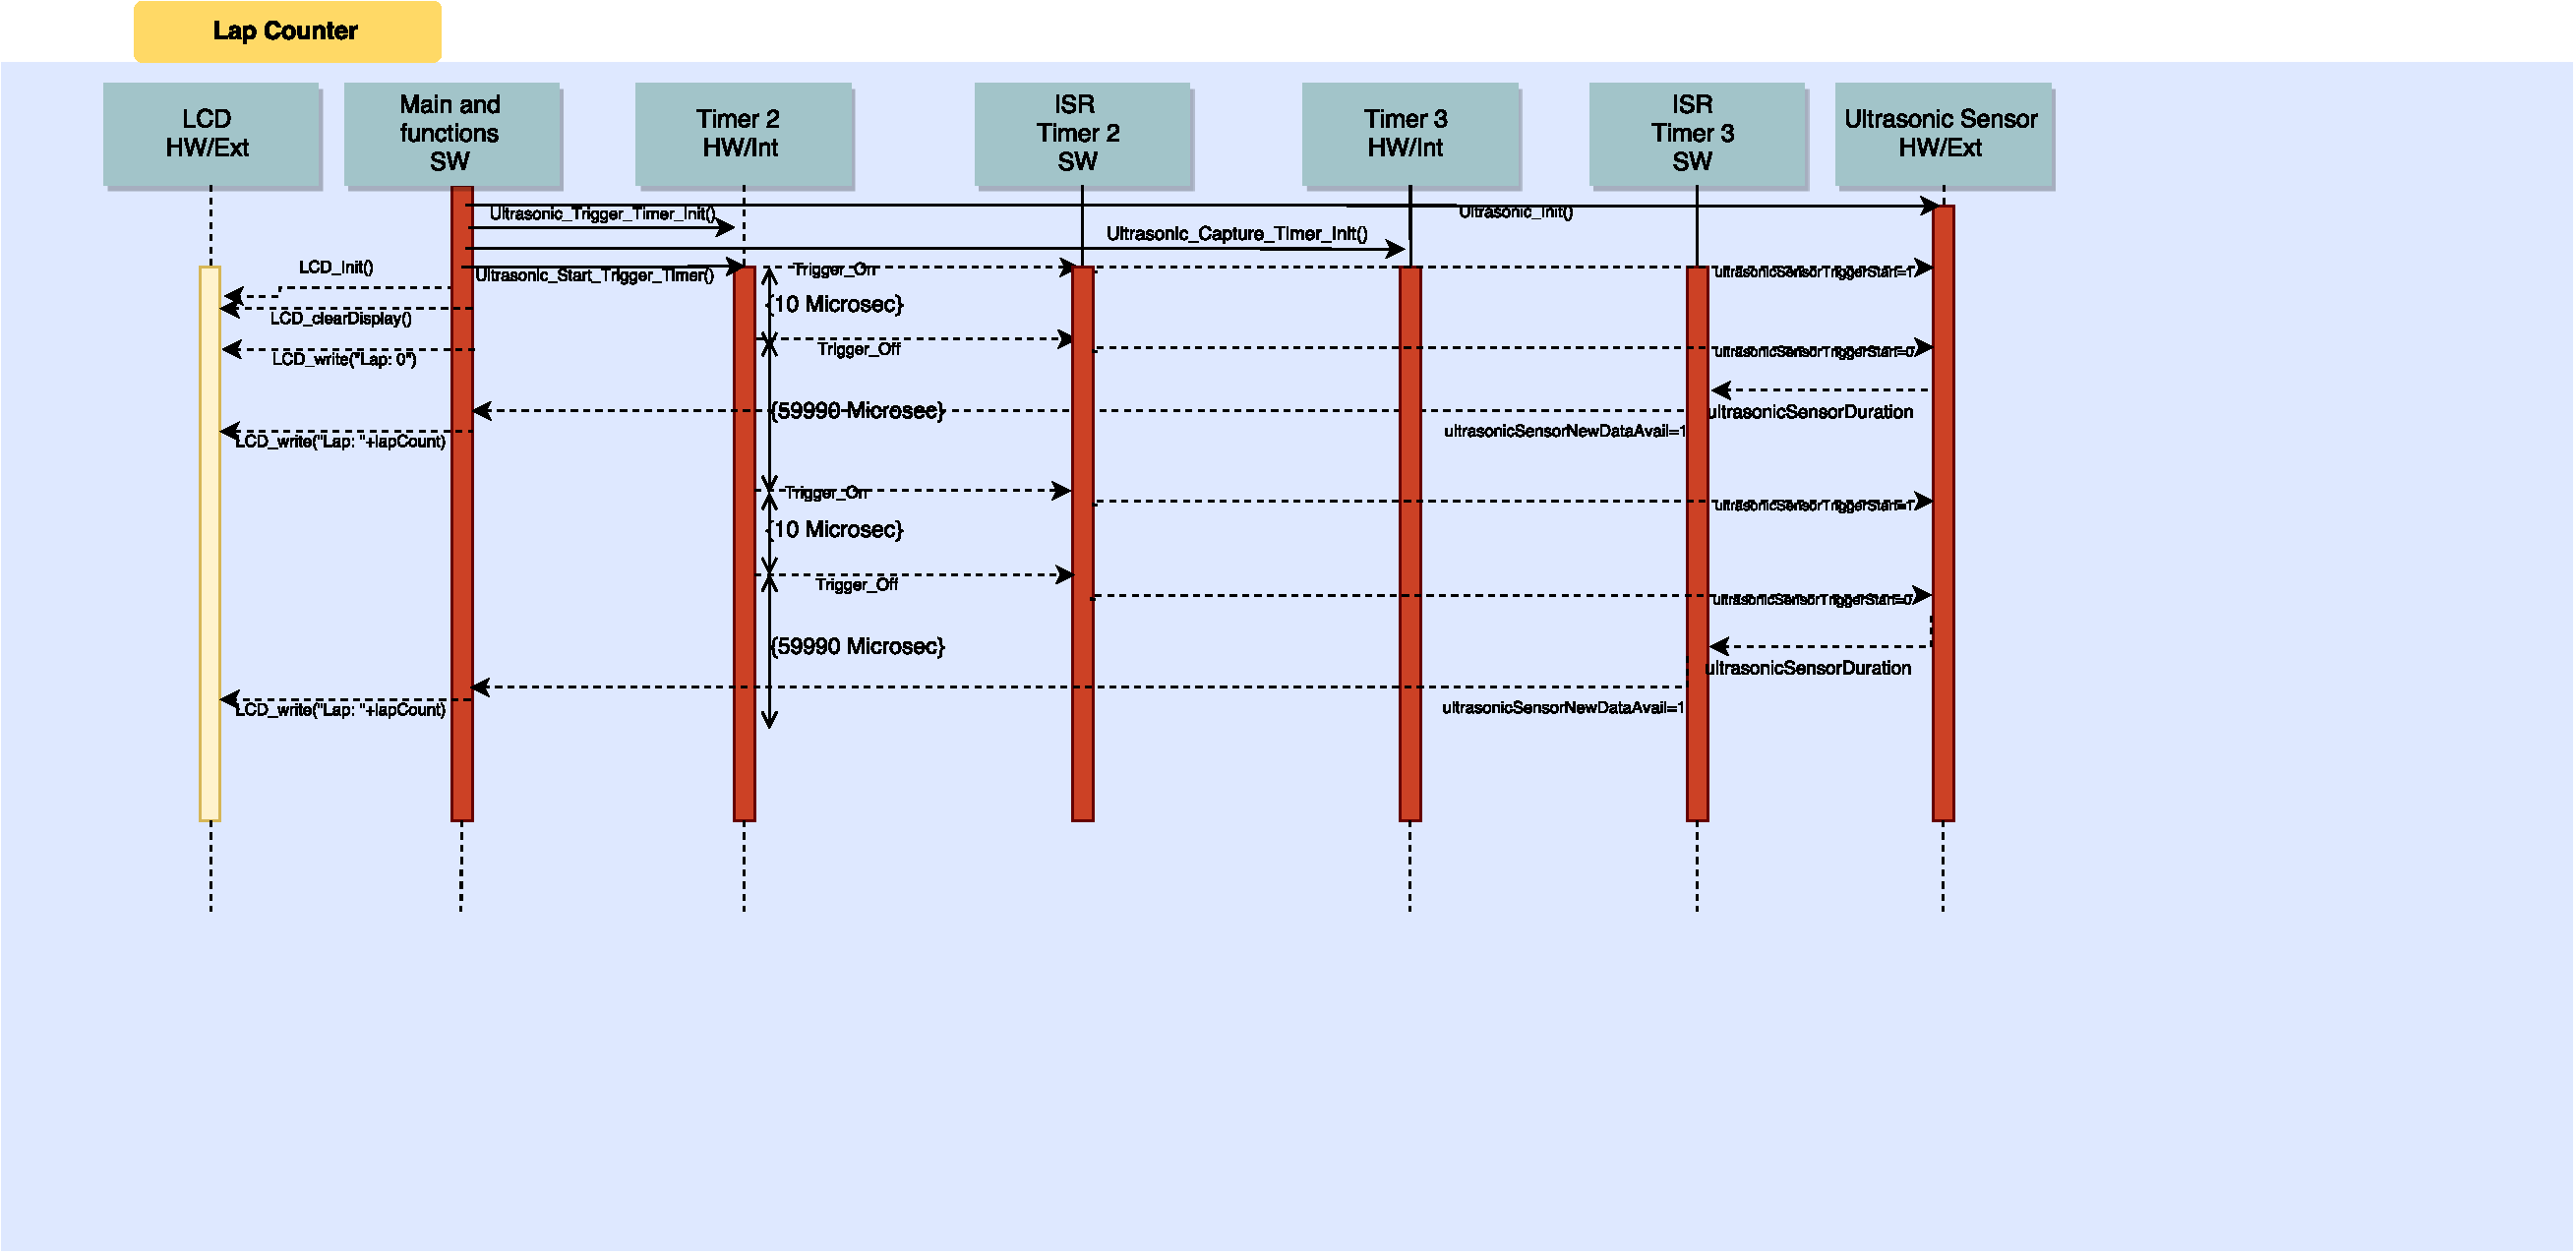
\includegraphics[scale=0.3]{Lap_Counter_Seq_Diagram}
\\
{\huge {Module: Getting Speed Data from Input Device}}
\\
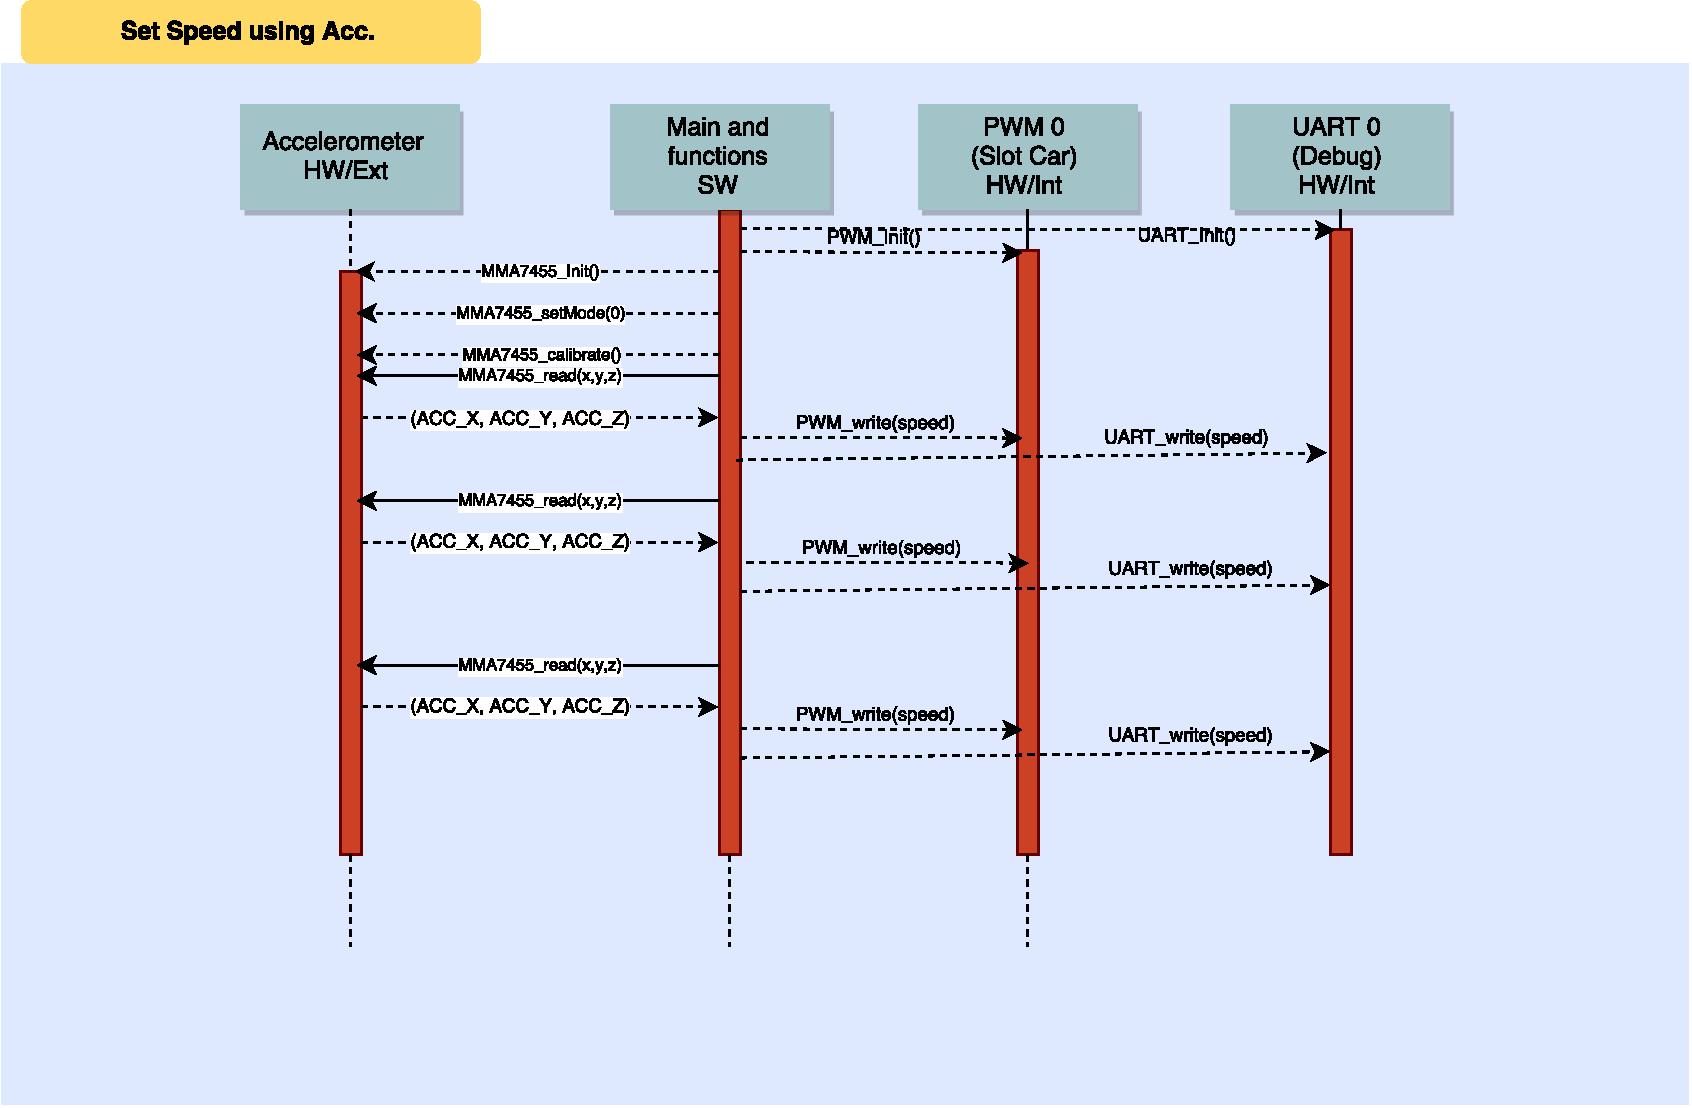
\includegraphics[scale=0.5]{Read_Acc_Control_Speed}
\clearpage
{\huge\textbf {4-Coding}}
\\
{\huge {Module: Lap Counter}}
\\
\begin{tabular}{| C{4cm} | C{4cm} | C{4cm} | C{2cm} |}
\hline
\textbf{Function Name} &\textbf{Function Definition}  & \textbf{Objective} &\textbf{WCET}\linebreak(simulation)\\
\hline
Ultrasonic\_Init() & Initialization of the Ultrasonic sensor. Functions of the trigger
and echo pins connected to the LPC board are defined in the IOCON registers& There are 2 data pins to
communicate with the ultrasonic sensor. Enabling the corresponding pins in the main board, their directions'
(input or output) is set for echo and trigger pins. So that, the board is able to trigger a calculation
of the distance and get the incoming signals with echo pin.& 18 usec\\
\hline
Ultrasonic\_Trigger\_Timer\_Init()&Trigger timer initializer. The output for the trigger pin is
 initialized in this function & Timer 2 is used to synchronize the value(either HIGH or LOW) to the Ultrasonic
 sensor. To initialized it, this function is used. First the power is enabled to this section with PCONP Register
 , then counters (Timer counters and Prescale counters) and match values are set appropriately. Last, the
 function on a match("toggle" in this case) is set. & 31 usec\\
\hline
LCD\_init()&Initialization of the LCD and its pins.& LCD is initialized by setting its pins' functionalities on the board,
and sending correct values to initialize the external driver, ( like 0x03, 0x03,0x03,0x02)&5.18 sec\\
\hline
\end{tabular}
\begin{tabular}{| C{4cm} | C{4cm} | C{4cm} | C{2cm} |}
\hline
Ultrasonic\_Capture\_Timer\_Init()& Echo timer initializer for the echo signal of the ultrasonic sensor.&
First the using PCONP register, the timer is powered on. Then its match registers and timer and prescale timer registers
are given the appropriate functionalities. This timer is used to count the elapsed time from the transmission of the
signals to the echo of the sent signals. So that, the distance of the object could be detected.&21.3 usec\\
\hline
Serial\_init()&Initialization of the UART 0 & Using UART(Serial communication), the debug information of distance of the detected object
and the lap count will be sent to the computer. &57.8 usec\\
\hline
TU()&Task for Ultrasonic, calculates the distance&The distance is calculated detected by ultrasonic sensor.
This distance is used to detect whether the car is in the range or not.&30.6 microsec\\
\hline
TC()& Task for the lap counter & After getting the distance detected, this function checks whether the
distance is smaller than the threshold, if it is, then the lap count is incremented by one. &23.0 microsec\\
\hline
TSD()&Task for system diagnosis, includes sending distance detected and the lap count data from UART
to PC & In order to debug the code, we are using this function which will be printing the value of
distance measured and the lap counted.&192 millisec\\
\hline
TDi()&This function sets the cursor to the appropriate position, then clears the display starting from the
cursor, then writes the lap count into the LCD screen.& To meet the requirements specified,
this function is used. It basically, writes the lap count into the LCD screen.&12.2 microsec\\
\hline
\end{tabular}
{\huge {Module: Getting Speed Data from Input Device}}
\\
\begin{tabular}{| C{4cm} | C{4cm} | C{4cm} | C{2cm} |}
\hline
\textbf{Function Name} &\textbf{Function Definition}  & \textbf{Objective} &\textbf{WCET}\linebreak(simulation)\\
\hline
TI()&Function initializes all the devices/modules used by the operating code.Basically consists of initializing
accelerometer, PWM pin, &In order to use the devices in the board, we have to initialize them before using.
Powering on the devices(PCONP) and giving the appropriate pin functionalities(IOCON) are done in this step.&5.86 secs\\
\hline
TSS()&Task for setting the speed of the car. To set a speed, first we are reading the angle of the board, from the
accelerometer. Using the angle value of it, the pulse width of the output signal is modulated from 0 to 999 where 500
means that 50\% duty cycle.& To meet the requirements specified, we are using the accelerometer data as input to
set the speed of the slot car. After getting the angle value, the speed of the car is set by using PWM.&44.6 microsec\\
\hline
TGA()&Task for getting the angle of the board using the accelerometer device on it. This function reads the
acceleration data from the device on the LPC board and finds the angle in the X dimension of the device.&
To make the speed of the slot car controllable by an input device, accelerometer device is used and according to
its angle in the X direction, the speed of the car is set. This function realizes the getting the angle data.&79.7 microsec\\
\hline
TSD()&Task for system diagnosis. This function is used to send the speed information to the PC using UART.&To debug the
code that we wrote in this section, the data produced is sent to the PC to oversee the system working.&522 millisec\\
\hline
\end{tabular}
\clearpage
{\huge\textbf {5-Scheduling}}
\\
{\huge {Module: Lap Counter}}
\\
In this part of the project, we are using Polling with interrupts. When a new data
is received using the ISR\_echoCaptureCounter, the flag ultrasonicSensorNewDataAvailable is
set to 1, the pseudo code is as follows:\\
ISR\_echoCaptureCounter()\{\\ if new data then\\ ultrasonicSensorDuration=duration;
ultrasonicSensorNewDataAvailable=1; \\
\}\\
This ISR is initiated after each 60 milliseconds and called when a signal is echoed back to the sensor.
This process of repeated initialization and waiting functions are done via the usage of Timer 2 and Timer 3
together.\\
While the ISR is not running, the main function polls the flag ultrasonicSensorNewDataAvailable.
The execution of the main loop is as follows:\\
while(true)\{\\
TU();//Poll the flag, if there is new data available, then calculate the distance\\
TC();//If the new distance is smaller then the threshold, increment the lap Counter\\
TDI();//Display the lap count value in the LCD\\
TSD();// System diagnosis, send relevant information using UART to debug\\
\}\\
\\
{\huge {Module: Getting Speed Data from Input Device}}
\\
In this section, there is no interrupt used, the code executes in a cycle and reads data from the
accelerometer. The communication with the accelerometer is done via I2C. An interrupt algorithm could have
been "Set a timer to repeat infinitely with a frequency, check if the value in accelerometer changed and
set a flag if it is changed.". However, this has no benefits over polling the data itself with a frequency,
so we decided that it is more convenient if it is not used. The main schedule of this module program is that:\\
while(true)\{\\
TGA();//Poll the value in accelerometer and calculate angle\\
TSS();//Set the speed of the car using the angle value from acc.\\
TSD();//Send the debug information to the PC\\
\}
\\[0.5in]
\begin{tabular}{| C{4cm} | C{4cm} | C{5cm} |}
\hline
Shared Variable&Name of the function&Name of the ISR\\
\hline
ultrasonicNewDataAvailable&TU& ISR\_echoCaptureCounter\\
\hline
ultrasonicSensorDuration&TU&ISR\_echoCaptureCounter\\
\hline
ultrasonicSensorTriggerStart&TI&ISR\_ultrasonicTriggerToggler\\
\hline
\end{tabular}
\clearpage
{\huge\textbf {6-Timing Diagram}}
\\
\includegraphics[scale=0.5]{Timing_Diagram}
\\
\begin{tabular}{| C{4cm} | C{4cm} | C{1cm} | C{2cm} | C{2cm} |}
\hline
Name of the ISR	 &	Shared Variable				&			Priority&	WCET	&	ACET\\
\hline
ISR\_ultrasonicTriggerToggler &	ultrasonicSensorTriggerStart		&			5	&	6.9 us	&	6.32 us\\
\hline
ISR\_echoCaptureCounter	& ultrasonicSensorDuration, ultrasonicSensorNewDataAvailable&	1	&	8.5 us&		6.1 us\\
\hline
\end{tabular}
\clearpage
{\huge\textbf {7-Hardware Block Diagram}}
\\
\begin{tabular}{| C{4cm} | C{4cm} | C{2cm} | C{2cm} | C{2cm} |}
\hline
Component &Type ID &Quickstart Board & Base-board & Off-board\\
\hline
Ultrasonic  &    HC-SR04  & &&                                             x\\
\hline
LCD       &      LCM-S01601DSR &&&                                         x\\
\hline
Potentiometre &  B10K  &&&                                                 x\\
\hline
Accelerometer &  MMA7455    & &                              X&\\
\hline
LED  &  &  &&                                                              X\\
\hline
1K-Resistor &&&&            X\\
\hline
\end{tabular}
\\[2in]
\begin{tabular}{| C{10cm} | C{2cm} |}
\hline
Expenses& Cost\\
\hline
120pcs 10cm male to male + male to female and female to female jumper wire&\$2.5\\
\hline
\end{tabular}
\clearpage
{\huge\textbf {8-Board Pin Table}}
\\[0.5in]
\begin{tabular}{| C{5cm} | C{5cm} |}
\hline
LCD PINS      &     LPC4088 PINS\\
\hline
1            &         GND\\
\hline
2            &         VU\\
\hline
3        &    to 2. pin of potentiometer\\
\hline
4 RS      &           P0.8 (P12)       \\
\hline
5 RW      &           P0.6 (P14) \\
\hline
6 EN       &          P0.7 (P13)\\
\hline
11 DATA0    &            P0.24 (P16)\\
\hline
12 DATA1     &           P0.25 (P17)\\
\hline
13 DATA2      &          P0.26 (P18)\\
\hline\\
14 DATA3       &         P1.30 (P19)\\
\hline
\end{tabular}
\\[1in]
\begin{tabular}{| C{5cm} | C{5cm} |}
\hline
Potentiometer&LPC4088 PINS\\
\hline
left & Vin\\
\hline
right & GND\\
\hline
\end{tabular}
\\[1in]
\begin{tabular}{| C{5cm} | C{5cm} |}
\hline
Ultrasonic&LPC4088 PINS\\
\hline
Vcc & Vin\\
\hline
GND & GND\\
\hline
Trig Trigger & P0.9(P11)\\
\hline
Echo Echo & P0.23(P15)\\
\hline
\end{tabular}
\\[1in]
\begin{tabular}{| C{5cm} | C{5cm} |}
\hline
Slot Car&LPC4088 PINS\\
\hline
Vcc & P1.5(P28)\\
\hline
GND & GND\\
\hline
\end{tabular}
\\
\clearpage
{\huge\textbf {9-Appendix}}
\\[0.5in]
Please see the LapCountModule and GettingSpeedFromInputModule folders for the
related source code.
\end{document}
